%% ShopSphere — Solution Proposal (Set-E: E-Commerce on AWS)
%% Compile: pdflatex proposal.tex  (run twice for TOC/references)
\documentclass[11pt,a4paper]{article}

\usepackage[T1]{fontenc}
\usepackage[utf8]{inputenc}
\IfFileExists{lmodern.sty}{\usepackage{lmodern}}{}
\usepackage[margin=2.2cm]{geometry}
\usepackage{xcolor}
\usepackage{graphicx}
\usepackage{float}
\usepackage{booktabs,tabularx,array,longtable,multirow}
\usepackage{enumitem}
\usepackage{tikz}
\usetikzlibrary{positioning,arrows.meta,fit,backgrounds,shapes.geometric,calc}
\usepackage{pgfgantt}
\usepackage{listings}
\usepackage{fancyhdr}
\usepackage{titlesec}
\usepackage[most]{tcolorbox}
\IfFileExists{xurl.sty}{\usepackage{xurl}}{}
\usepackage[hidelinks]{hyperref}

% ---------- colours (match DESIGN.md) ----------
\definecolor{primary}{HTML}{4F46E5}
\definecolor{accent}{HTML}{F59E0B}
\definecolor{dsrds}{HTML}{2563EB}
\definecolor{dswriter}{HTML}{7C3AED}
\definecolor{dsreader}{HTML}{0D9488}
\definecolor{dsddb}{HTML}{EA580C}
\definecolor{ink}{HTML}{0F172A}
\definecolor{muted}{HTML}{64748B}
\definecolor{soft}{HTML}{F1F5F9}

% ---------- placeholders: EDIT THESE ----------
\newcolumntype{Y}{>{\raggedright\arraybackslash}X}
\newcommand{\memberA}{Sudeep Kumar Sahu}
\newcommand{\rollA}{24BCT0160}
\newcommand{\memberB}{Shrijay Sinha}
\newcommand{\rollB}{24BCE2998}
\newcommand{\course}{Cloud Architecture Design}
\newcommand{\faculty}{Prof. Sudhakar P}
\newcommand{\institute}{Vellore Instituteof Technology}
\newcommand{\awsregion}{Vellore}

\titleformat{\section}{\large\bfseries\color{primary}}{\thesection}{0.6em}{}
\titleformat{\subsection}{\normalsize\bfseries\color{ink}}{\thesubsection}{0.6em}{}
\setlist{itemsep=2pt,topsep=4pt}
\setlength{\parskip}{4pt}
\setlength{\parindent}{0pt}

\pagestyle{fancy}
\fancyhf{}
\lhead{\small\color{muted}ShopSphere -- Solution Proposal}
\rhead{\small\color{muted}Set-E: E-Commerce on AWS}
\cfoot{\small\thepage}
\renewcommand{\headrulewidth}{0.3pt}

\lstset{basicstyle=\ttfamily\footnotesize,breaklines=true,frame=single,
  rulecolor=\color{muted!40},backgroundcolor=\color{soft},columns=fullflexible,
  keywordstyle=\color{primary}\bfseries,commentstyle=\color{muted},
  aboveskip=6pt,belowskip=6pt}

\newtcolorbox{keybox}[1]{colback=soft,colframe=primary,fonttitle=\bfseries,
  title=#1,boxrule=0.6pt,arc=2mm,left=6pt,right=6pt,top=4pt,bottom=4pt}

\begin{document}

% ======================= TITLE PAGE =======================
\begin{titlepage}
\centering
\vspace*{1.5cm}
{\color{muted}\large \institute\par}
\vspace{0.4cm}
{\color{muted}\course\par}
\vspace{2cm}
{\Huge\bfseries\color{primary} ShopSphere\par}
\vspace{0.3cm}
{\Large A Multi-Database E-Commerce Platform on AWS\par}
\vspace{0.3cm}
{\large\color{muted} Amazon RDS \textbullet{} Amazon Aurora \textbullet{} Amazon DynamoDB\par}
\vspace{1.2cm}
{\large\bfseries Solution Proposal -- Assignment Set-E\par}
\vspace{2cm}
\begin{tabular}{@{}lll@{}}
\toprule
\textbf{Member} & \textbf{Registration No.} & \textbf{Role}\\
\midrule
\memberA & \rollA & Relational \& Data Lead\\
\memberB & \rollB & Application, NoSQL \& Cloud Lead\\
\bottomrule
\end{tabular}

\vfill
Submitted to: \textbf{\faculty}\\[4pt]
\end{titlepage}

% ======================= ABSTRACT =======================
\begin{abstract}
\noindent We propose \textbf{ShopSphere}, a working online shop deployed on Amazon Web Services in which customers register and log in, browse products, manage a cart, place orders, pay and track deliveries. Rather than forcing all data into one database, ShopSphere places each kind of data in the AWS database whose model matches its access pattern: \textbf{Amazon RDS for PostgreSQL} stores customers, products, orders and payments with full ACID guarantees; \textbf{Amazon Aurora PostgreSQL} hosts the same relational schema during a simulated festival sale, separating write traffic (orders) from read traffic (browsing) across instances in different Availability Zones; and \textbf{Amazon DynamoDB} keeps shopping carts, login sessions and user preferences as key-value documents. A runtime switch moves the application from RDS to Aurora without redeployment, and every screen displays which database and which instance served it, so each architectural claim can be verified live in the AWS Management Console. The design targets near-zero cost (a few dollars of AWS Free Tier credits) and is planned for a two-member team with clearly separated ownership.
\end{abstract}

\tableofcontents
\newpage

% ======================= 1 =======================
\section{Problem Statement}
An e-commerce application must support six customer capabilities: \emph{register and log in, browse products, add products to a cart, place orders, make payments and track orders}. The underlying data is not uniform:
\begin{itemize}
  \item \textbf{Customers $\rightarrow$ Orders $\rightarrow$ Order Items $\rightarrow$ Products} form a chain of one-to-many relationships involving money and inventory. Integrity (no order without a customer, no payment without an order, no negative stock) is mandatory.
  \item During a \textbf{festival sale}, traffic can rise from about 1{,}000 to more than 100{,}000 concurrent users, and the increase is dominated by \emph{reads} (browsing), while \emph{writes} (orders) must remain correct and available.
  \item The \textbf{shopping cart}, \textbf{sessions} and \textbf{preferences} are small per-customer documents read and written on almost every click, always by a single key, and never joined with other data.
\end{itemize}
The assignment asks us to implement this use case on AWS, demonstrate that it works, and compare Amazon RDS, Amazon Aurora and Amazon DynamoDB.

% ======================= 2 =======================
\section{Objectives}
\begin{enumerate}[label=\textbf{O\arabic*}]
  \item Deliver all six customer capabilities as a working web application on AWS.
  \item Use \textbf{RDS} as the relational system of record and run the SQL queries given in the brief, unchanged, against application-generated data.
  \item Demonstrate \textbf{Aurora}'s advantages for the festival scenario: writer/reader separation, read scaling, serverless capacity scaling and automatic failover.
  \item Use \textbf{DynamoDB} for the cart (keyed by customer id, exactly the document shape in the brief), sessions (with automatic expiry) and preferences.
  \item Produce an evidence-based comparison of the three services.
  \item Keep AWS spending to a few dollars of Free Tier credits and delete all resources after the demonstration.
\end{enumerate}

% ======================= 3 =======================
\section{Proposed Solution Overview}
ShopSphere is a single web application (React front end served by a Node.js/Express API) running on one small Amazon EC2 instance. The API talks to three data stores and routes every operation explicitly. Table~\ref{tab:mapping} maps each customer capability to its data store.

\begin{table}[H]
\centering\small
\begin{tabularx}{\linewidth}{@{}l X l@{}}
\toprule
\textbf{Capability} & \textbf{Implementation} & \textbf{Data store}\\
\midrule
Register / log in & bcrypt-hashed password in \texttt{customers}; session item with TTL; JWT cookie carries only the session id & RDS/Aurora + DynamoDB\\
Browse products & paginated search, filter, sort & RDS / \textbf{Aurora reader}\\
Cart & one document per customer, optimistic locking via a \texttt{version} attribute & \textbf{DynamoDB}\\
Place order & single ACID transaction with row locks on stock & RDS / \textbf{Aurora writer}\\
Payment & deterministic mock gateway, idempotency key, transactional status update & RDS / Aurora writer\\
Track order & status timeline from \texttt{order\_status\_history} & RDS / Aurora writer\\
\bottomrule
\end{tabularx}
\caption{Capability-to-database mapping}
\label{tab:mapping}
\end{table}

\begin{keybox}{Design idea that makes the demonstration verifiable}
Every API response carries headers naming the data source, role and instance (for example \texttt{Aurora $\cdot$ reader $\cdot$ shopsphere-aurora-reader-1 $\cdot$ 4\,ms}). The UI shows these as coloured badges. An evaluator can therefore watch browsing traffic go to the Aurora reader and orders go to the writer, then confirm the same instances in the console.
\end{keybox}

% ======================= 4 =======================
\section{System Architecture}

\begin{figure}[H]
\centering
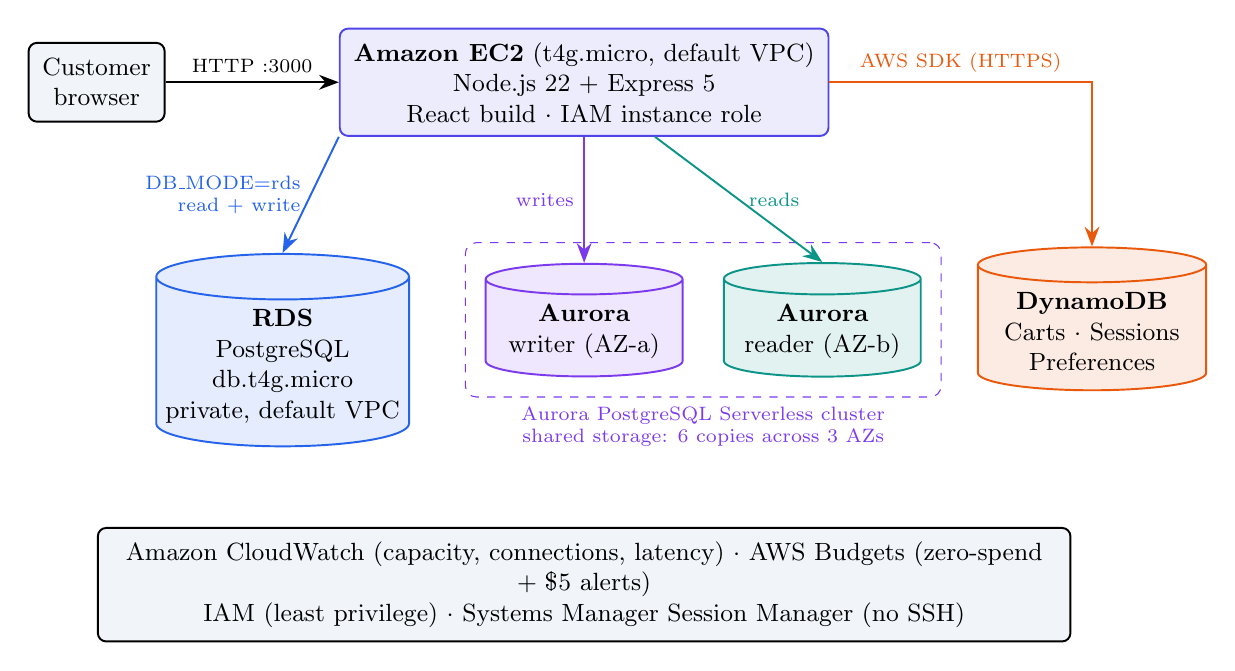
\begin{tikzpicture}[
  font=\small,
  box/.style={draw, rounded corners=3pt, align=center, minimum height=1cm, inner sep=5pt, line width=0.7pt},
  db/.style={cylinder, shape border rotate=90, aspect=0.18, draw, align=center, minimum width=2.5cm, minimum height=1.3cm, line width=0.7pt},
  arr/.style={-{Stealth[length=2.5mm]}, line width=0.7pt},
  node distance=0.9cm and 1.0cm]

\node[box, fill=soft] (user) {Customer\\browser};
\node[box, fill=primary!10, draw=primary, right=2.2cm of user, minimum width=4.4cm] (ec2) {\textbf{Amazon EC2} (t4g.micro, default VPC)\\Node.js 22 + Express 5\\React build $\cdot$ IAM instance role};

\node[db, fill=dsrds!12, draw=dsrds, below left=1.6cm and -0.6cm of ec2] (rds) {\textbf{RDS}\\PostgreSQL\\db.t4g.micro\\private, default VPC};
\node[db, fill=dswriter!12, draw=dswriter, below=1.6cm of ec2] (aw) {\textbf{Aurora}\\writer (AZ-a)};
\node[db, fill=dsreader!12, draw=dsreader, right=0.5cm of aw] (ar) {\textbf{Aurora}\\reader (AZ-b)};
\node[db, fill=dsddb!12, draw=dsddb, right=0.7cm of ar, minimum width=2.9cm] (ddb) {\textbf{DynamoDB}\\Carts $\cdot$ Sessions\\Preferences};

\begin{scope}[on background layer]
\node[draw=dswriter, dashed, rounded corners, fit=(aw)(ar), inner sep=7pt, label={[font=\scriptsize,text=dswriter,align=center]below:Aurora PostgreSQL Serverless cluster\\shared storage: 6 copies across 3 AZs}] (cl) {};
\end{scope}

\draw[arr] (user) -- node[above,font=\scriptsize]{HTTP :3000} (ec2);
\draw[arr, dsrds] (ec2.south west) -- node[left,font=\scriptsize,align=right]{DB\_MODE=rds\\read + write} (rds.north);
\draw[arr, dswriter] (ec2.south) -- node[left,font=\scriptsize]{writes} (aw.north);
\draw[arr, dsreader] ($(ec2.south)+(0.9,0)$) -- node[right,font=\scriptsize]{reads} (ar.north);
\draw[arr, dsddb] (ec2.east) -| node[above,pos=0.25,font=\scriptsize]{AWS SDK (HTTPS)} (ddb.north);

\node[box, fill=soft, below=1.9cm of aw, text width=12cm] (cw) {\centering Amazon CloudWatch (capacity, connections, latency) $\cdot$ AWS Budgets (zero-spend + \$5 alerts)\\ IAM (least privilege) $\cdot$ Systems Manager Session Manager (no SSH)};
\end{tikzpicture}
\caption{ShopSphere deployment architecture}
\label{fig:arch}
\end{figure}

\textbf{Components.}
\begin{itemize}
  \item \textbf{EC2 application server} in the default VPC's public subnet, managed by \texttt{pm2}. Shell access through AWS Systems Manager Session Manager (no SSH port open). AWS credentials come from an IAM instance role; no access keys are stored on the server.
  \item \textbf{Amazon RDS for PostgreSQL}: single-AZ \texttt{db.t4g.micro}, not publicly accessible; its security group accepts port 5432 only from the application's security group. Represents normal-traffic operation.
  \item \textbf{Amazon Aurora PostgreSQL (serverless)}: one writer and one reader placed in different Availability Zones, capacity range 0--2 ACU, created with Aurora's express configuration (the option available on the AWS Free plan), which exposes the cluster through an IAM-authenticated internet access gateway. Represents festival-sale operation.
  \item \textbf{Amazon DynamoDB}: three on-demand tables (\texttt{ShopSphere\_Carts}, \texttt{ShopSphere\_Sessions} with Time-to-Live, \texttt{ShopSphere\_UserPreferences}).
\end{itemize}

\textbf{Read/write routing.} All SQL calls go through \texttt{db.read()} or \texttt{db.write()}. In RDS mode both resolve to the single instance; in Aurora mode \texttt{read} uses the reader endpoint and \texttt{write} the cluster (writer) endpoint. Catalog browsing and reports are reads; registration, checkout, payment and a customer's own order history use the writer so that a customer always sees what they just wrote (read-your-writes).

% ======================= 5 =======================
\section{Database Design}

\subsection{Relational model (RDS and Aurora)}
The same PostgreSQL schema is used on RDS and Aurora. Customer identifiers start at 101 and product identifiers follow the brief (\texttt{P100}, \texttt{P200}, \dots) so that the queries and documents in the assignment work unmodified.

\begin{figure}[H]
\centering
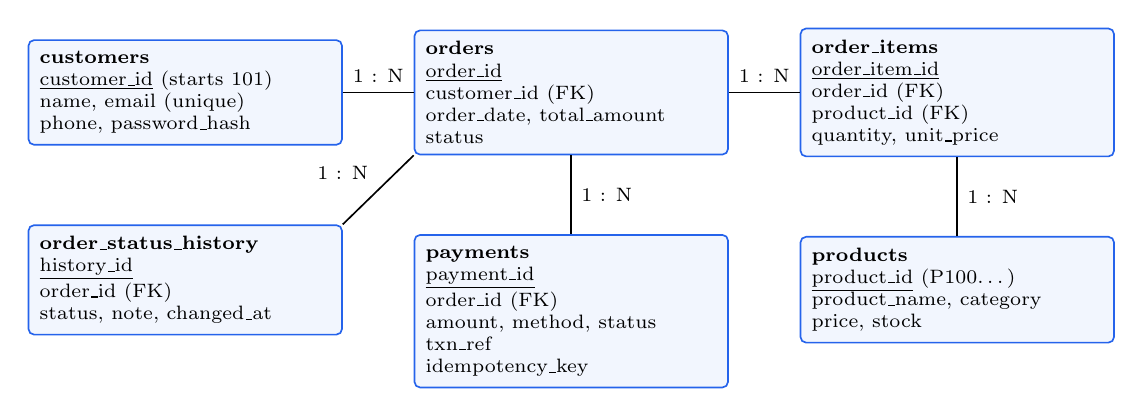
\begin{tikzpicture}[font=\scriptsize,
  ent/.style={draw=dsrds, line width=0.6pt, rounded corners=2pt, align=left, fill=dsrds!6, inner sep=4pt, text width=3.7cm},
  rel/.style={line width=0.6pt}]
\node[ent] (c) {\textbf{customers}\\ \underline{customer\_id} (starts 101)\\ name, email (unique)\\ phone, password\_hash};
\node[ent, right=0.9cm of c] (o) {\textbf{orders}\\ \underline{order\_id}\\ customer\_id (FK)\\ order\_date, total\_amount\\ status};
\node[ent, right=0.9cm of o] (oi) {\textbf{order\_items}\\ \underline{order\_item\_id}\\ order\_id (FK)\\ product\_id (FK)\\ quantity, unit\_price};
\node[ent, below=1.0cm of oi] (p) {\textbf{products}\\ \underline{product\_id} (P100\dots)\\ product\_name, category\\ price, stock};
\node[ent, below=1.0cm of o] (pay) {\textbf{payments}\\ \underline{payment\_id}\\ order\_id (FK)\\ amount, method, status\\ txn\_ref\\ idempotency\_key};
\node[ent, below=1.0cm of c] (h) {\textbf{order\_status\_history}\\ \underline{history\_id}\\ order\_id (FK)\\ status, note, changed\_at};
\draw[rel] (c) -- node[above]{1 : N} (o);
\draw[rel] (o) -- node[above]{1 : N} (oi);
\draw[rel] (p) -- node[right]{1 : N} (oi);
\draw[rel] (o) -- node[right]{1 : N} (pay);
\draw[rel] (o.south west) -- node[above left]{1 : N} (h.north east);
\end{tikzpicture}
\caption{Entity-relationship model}
\end{figure}

Integrity is enforced by the database itself: primary and foreign keys, \texttt{UNIQUE(email)}, \texttt{CHECK (stock >= 0)}, \texttt{CHECK} constraints on status values, \texttt{NUMERIC} types for money and a unique idempotency key on payments.

\subsection{Checkout as one ACID transaction}
\begin{lstlisting}[language=SQL]
BEGIN;
SELECT product_id, price, stock FROM products
 WHERE product_id = ANY($1) ORDER BY product_id FOR UPDATE;   -- lock rows in fixed order
-- application verifies stock >= quantity for every line, else ROLLBACK
INSERT INTO orders (customer_id, total_amount, status) VALUES ($2, $3, 'PLACED') RETURNING order_id;
INSERT INTO order_items (order_id, product_id, quantity, unit_price) VALUES (...);
UPDATE products SET stock = stock - $q WHERE product_id = $p;   -- per line
INSERT INTO order_status_history (order_id, status) VALUES ($id, 'PLACED');
COMMIT;   -- only now is the DynamoDB cart deleted
\end{lstlisting}
If any product lacks stock, the whole transaction rolls back: no order, no items, no stock change. This is demonstrated live with a low-stock product.

\subsection{Festival sale on Aurora}
\begin{itemize}
  \item \textbf{Read scaling:} browsing (the bulk of festival traffic) is served by the reader; the writer handles only orders and payments. Aurora replicas share the cluster storage volume, so adding a reader does not copy data and replica lag stays low.
  \item \textbf{Elastic capacity:} each serverless instance scales in Aurora Capacity Units between 0 and 2 ACU and pauses when idle, so cost follows traffic.
  \item \textbf{Availability:} writer and reader sit in different Availability Zones; a manual failover promotes the reader, the cluster endpoint follows the new writer, and the application reconnects without a restart.
  \item \textbf{Migration:} the RDS database is copied to Aurora with \texttt{pg\_dump}/\texttt{psql}; because both are PostgreSQL, no schema or query changes are required.
\end{itemize}

\subsection{NoSQL model (DynamoDB)}
\begin{table}[H]
\centering\small
\begin{tabularx}{\linewidth}{@{}l l l X@{}}
\toprule
\textbf{Table} & \textbf{Partition key} & \textbf{TTL} & \textbf{Access pattern}\\
\midrule
ShopSphere\_Carts & customer\_id & -- & GetItem / conditional PutItem / DeleteItem by customer\\
ShopSphere\_Sessions & session\_id & expires\_at & PutItem at login, GetItem per request, DeleteItem at logout\\
ShopSphere\_UserPreferences & customer\_id & -- & GetItem / UpdateItem (theme, categories, recently viewed)\\
\bottomrule
\end{tabularx}
\caption{DynamoDB tables (on-demand capacity)}
\end{table}

The cart item for customer 101 is exactly the document given in the brief, plus a version number used for optimistic concurrency control:
\begin{lstlisting}
{ "customer_id": "101",
  "items": [ { "product_id": "P100", "quantity": 2 },
             { "product_id": "P200", "quantity": 1 } ],
  "version": 7 }
\end{lstlisting}
A cart is fetched with a single \texttt{GetItem} on \texttt{customer\_id = "101"}: no SQL, no joins and no table scans. Session items expire automatically through DynamoDB Time-to-Live, and the application also checks the expiry timestamp because TTL deletion is not instantaneous.

% ======================= 6 =======================
\section{Comparison of RDS, Aurora and DynamoDB}

\begin{table}[H]
\centering\footnotesize
\renewcommand{\arraystretch}{1.25}
\begin{tabularx}{\linewidth}{@{}>{\bfseries\raggedright\arraybackslash}p{2.3cm} Y Y Y@{}}
\toprule
Feature & \textbf{\color{dsrds}Amazon RDS} & \textbf{\color{dswriter}Amazon Aurora} & \textbf{\color{dsddb}Amazon DynamoDB}\\
\midrule
Database type & Relational (managed MySQL, PostgreSQL, MariaDB, Oracle, SQL Server) & Relational, cloud-native distributed storage (MySQL/PostgreSQL compatible) & NoSQL key-value and document\\
SQL & Yes, full SQL & Yes, full SQL & No SQL engine; key-based API plus PartiQL (SQL-like, single table)\\
JOINs & Yes & Yes & No; data is modelled per access pattern (denormalised)\\
Flexible schema & No; fixed columns, changed with \texttt{ALTER TABLE} (JSONB columns help) & No; same as RDS & Yes; only key attributes are fixed\\
Serverless options & No; an instance size is chosen & Yes; Aurora Serverless scales in ACUs and can pause at zero & Yes; fully serverless, on-demand capacity\\
Very large scale & Moderate; vertical scaling and asynchronous read replicas & High; up to 15 low-lag readers on shared storage replicated six ways across three AZs & Very high; virtually unlimited throughput and storage with consistent millisecond latency\\
Transactions & Full ACID, multi-table & Full ACID, multi-table & ACID transactions across up to 100 items (\texttt{TransactWriteItems})\\
High availability & Optional Multi-AZ standby (extra cost) & Fast failover by promoting a reader & Built in, multi-AZ by default\\
Cost model & Instance hours + storage; cheapest for small steady loads & ACU-hours (serverless) or instance hours, plus storage and I/O & Per request (on-demand) or provisioned capacity, plus storage\\
\midrule
Best for & Customer and order management at normal traffic & The same relational workload at festival scale: read-heavy spikes and high availability & Shopping carts, sessions and preferences: single-key, high-frequency access\\
\bottomrule
\end{tabularx}
\caption{Feature comparison (completed table from the brief)}
\label{tab:compare}
\end{table}

\textbf{Evidence in the demonstration.} JOINs and transactions are shown with the brief's SQL and the checkout rollback on RDS; read scaling, serverless capacity and failover are shown on the Aurora cluster and CloudWatch; flexible schema and key-based access are shown with the cart document and PartiQL in the DynamoDB console. An \emph{Insights} page reports measured median latencies for a DynamoDB \texttt{GetItem}, an Aurora reader query and a writer query, giving the comparison a quantitative element.

% ======================= 7 =======================
\section{Security Design}
\begin{itemize}
  \item \textbf{Network:} RDS is private and reachable only from the application security group; the EC2 instance exposes only the application port; no SSH port is opened (Session Manager is used instead).
  \item \textbf{Identity:} the application uses an IAM instance role restricted to the three ShopSphere tables and to \texttt{rds-db:connect} for one database user on the Aurora cluster. Aurora connections use short-lived IAM authentication tokens instead of stored passwords.
  \item \textbf{Data in transit and at rest:} TLS for all database connections; storage encryption enabled on RDS, Aurora and DynamoDB.
  \item \textbf{Application:} parameterised SQL only, input validation, bcrypt password hashing, httpOnly session cookies with server-side revocation, rate limiting on login, a least-privilege database role, and no full card numbers stored.
\end{itemize}

% ======================= 8 =======================
\section{Cost Analysis and Optimisation}
New AWS accounts on the Free plan receive promotional credits, and Aurora PostgreSQL serverless is available on that plan within fixed limits (up to 4 ACUs and 1\,GiB storage per cluster). We therefore expect \textbf{no out-of-pocket cost}. Development is done locally with Docker (PostgreSQL and DynamoDB Local), so AWS resources run for only about three days.

\begin{table}[H]
\centering\small
\begin{tabularx}{\linewidth}{@{}X l r@{}}
\toprule
\textbf{Resource} & \textbf{Configuration} & \textbf{Approx. 3-day cost}\\
\midrule
EC2 + public IPv4 + 10\,GB gp3 & t4g.micro & \$1.00\\
RDS for PostgreSQL & db.t4g.micro, Single-AZ, 20\,GB & \$1.40\\
Aurora PostgreSQL serverless & writer + reader, 0--2 ACU, auto-pause & \$1--2\\
DynamoDB & 3 on-demand tables & $<$\$0.05\\
CloudWatch, Budgets & basic metrics, 1 dashboard, 2 budgets & \$0\\
\midrule
\textbf{Total (paid from credits)} & & \textbf{\$3--6}\\
\bottomrule
\end{tabularx}
\caption{Estimated consumption (approximate on-demand rates; verified in the console before creation)}
\end{table}

Cost controls: zero-spend and monthly budgets with e-mail alerts; no NAT gateway, load balancer, Elastic IP or Multi-AZ RDS; Aurora pauses at zero capacity when idle; resources tagged \texttt{Project=ShopSphere} and stopped every evening; complete teardown immediately after recording, verified with Tag Editor and the billing console.

% ======================= 9 =======================
\section{Demonstration Plan}
The video (target 16 minutes, within the 10--20 minute limit) shows both members on camera alongside the AWS Management Console.

\begin{table}[H]
\centering\small
\begin{tabularx}{\linewidth}{@{}l l l X@{}}
\toprule
\textbf{\#} & \textbf{Time} & \textbf{Presenter} & \textbf{Content}\\
\midrule
1 & 0:00--1:00 & Both & Introductions, problem, solution in one sentence\\
2 & 1:00--2:30 & \memberB & Architecture walk-through, cost guardrails (Budgets)\\
3 & 2:30--5:00 & \memberB & Register/login (session in DynamoDB), browse, cart document and PartiQL\\
4 & 5:00--8:00 & \memberA & RDS configuration, brief's SQL queries, live order, rollback on low stock\\
5 & 8:00--9:15 & \memberB & Declined then successful payment, order tracking timeline\\
6 & 9:15--12:45 & \memberA & Aurora cluster, read-only reader proof, RDS$\rightarrow$Aurora switch, festival load test with CloudWatch\\
7 & 12:45--13:45 & \memberA & Manual failover and recovery\\
8 & 13:45--15:15 & \memberB & Measured latencies and the comparison table\\
9 & 15:15--16:00 & Both & Credits used, teardown, contributions, conclusion\\
\bottomrule
\end{tabularx}
\caption{Video outline}
\end{table}

% ======================= 10 =======================
\section{Team Roles and Contribution}
\begin{table}[H]
\centering\small
\begin{tabularx}{\linewidth}{@{}l X X@{}}
\toprule
\textbf{Area} & \textbf{\memberA} (Relational \& Data Lead) & \textbf{\memberB} (Application, NoSQL \& Cloud Lead)\\
\midrule
AWS services & RDS, Aurora cluster and reader, migration, failover drill & DynamoDB, EC2, IAM role and policies, security groups, Budgets, CloudWatch\\
Backend & Connection pools and read/write routing, IAM token auth, products, checkout transaction, payments, insights API & Authentication and sessions, cart with optimistic locking, preferences, middleware and data-source headers\\
Frontend & Admin API integration & All pages, components and design system\\
Documentation & Architecture and database design, this proposal & Requirements, UI design, AWS setup guide, demo script\\
Video & Segments 4, 6, 7 ($\approx$ 8 min) & Segments 2, 3, 5, 8 ($\approx$ 8 min)\\
\bottomrule
\end{tabularx}
\caption{Division of work}
\end{table}

Both members review each other's pull requests, so each understands the full system and can answer questions on any part.

% ======================= 11 =======================
\section{Timeline}
\begin{center}
\begin{ganttchart}[
  hgrid, vgrid,
  x unit=1.05cm, y unit chart=0.55cm,
  title height=1,
  bar/.append style={fill=primary!70, draw=primary},
  milestone/.append style={fill=accent, draw=accent},
  bar label font=\small, title label font=\small\bfseries
]{1}{9}
\gantttitle{Day}{9}\\
\gantttitlelist{1,...,9}{1}\\
\ganttbar{P0 Kick-off \& guardrails}{1}{1}\\
\ganttbar{P1 Local foundation}{1}{2}\\
\ganttbar{P2 Core features (local)}{2}{5}\\
\ganttbar{P3 AWS baseline}{6}{6}\\
\ganttbar{P4 Aurora festival mode}{6}{7}\\
\ganttbar{P5 Insights \& comparison}{7}{7}\\
\ganttbar{P6 Hardening \& rehearsal}{8}{8}\\
\ganttbar{P7 Recording \& report}{8}{9}\\
\ganttmilestone{P8 Teardown}{9}
\end{ganttchart}
\end{center}

% ======================= 12 =======================
\section{Risks and Mitigation}
\begin{table}[H]
\centering\small
\begin{tabularx}{\linewidth}{@{}X X@{}}
\toprule
\textbf{Risk} & \textbf{Mitigation}\\
\midrule
Credits consumed by forgotten resources & Budgets with alerts, nightly stop routine, tagged resources, teardown checklist\\
Aurora resumes slowly from zero capacity during recording & Minimum capacity raised to 0.5 ACU shortly before recording\\
IAM database authentication misconfiguration & Connection tested from CloudShell first; fallback to console-based SQL demonstration\\
Small instance runs out of memory during build & Swap file configured at launch\\
Video exceeds 20 minutes & Timed rehearsals and a prepared cut list\\
\bottomrule
\end{tabularx}
\caption{Risk register}
\end{table}

% ======================= 13 =======================
\section{Expected Outcomes and Future Scope}
\textbf{Outcomes:} a deployed shop covering all six capabilities; live proof of relational integrity on RDS, read/write separation, elastic capacity and failover on Aurora, and key-value access on DynamoDB; a completed, evidence-backed comparison; and a cost record showing the whole exercise ran on a few dollars of credits.

\textbf{Future scope:} Amazon Cognito for identity, a real payment gateway, Amazon CloudFront and S3 for static assets, DynamoDB Streams to publish order events, Aurora reader auto scaling, and infrastructure as code (AWS CDK) for repeatable environments.

% ======================= 14 =======================
\section{Conclusion}
ShopSphere shows that the question is not which AWS database is best, but which is best \emph{for each part of the data}. Relational integrity belongs in RDS; the same relational workload under festival-scale, read-heavy traffic benefits from Aurora's shared storage, readers and serverless scaling; and per-customer cart and session documents are served most simply and scalably by DynamoDB. The proposed implementation makes each of these choices visible and verifiable in a single working application, at negligible cost, with a clear and balanced division of work between the two team members.

% ======================= REFERENCES =======================
\section*{References}
\begin{enumerate}[label={[\arabic*]},leftmargin=*]
  \item Amazon RDS User Guide. \url{https://docs.aws.amazon.com/AmazonRDS/latest/UserGuide/}
  \item Amazon Aurora User Guide -- Aurora Serverless, endpoints, failover. \url{https://docs.aws.amazon.com/AmazonRDS/latest/AuroraUserGuide/}
  \item Amazon Aurora -- Create with express configuration. \url{https://docs.aws.amazon.com/AmazonRDS/latest/AuroraUserGuide/CHAP_GettingStartedAurora.AuroraPostgreSQL.ExpressConfig.html}
  \item Amazon Aurora on the AWS Free Tier. \url{https://docs.aws.amazon.com/AmazonRDS/latest/AuroraUserGuide/aurora-free-tier.html}
  \item Amazon DynamoDB Developer Guide -- core components, TTL, transactions, PartiQL. \url{https://docs.aws.amazon.com/amazondynamodb/latest/developerguide/}
  \item AWS Free Tier. \url{https://aws.amazon.com/free/}
  \item IAM database authentication for Aurora. \url{https://docs.aws.amazon.com/AmazonRDS/latest/AuroraUserGuide/UsingWithRDS.IAMDBAuth.html}
\end{enumerate}

\end{document}
